\documentclass[border=6pt]{standalone}
\usepackage{tikz}
\usepackage{pgfplots}
\pgfplotsset{compat=1.18}
\usetikzlibrary{arrows.meta,positioning,shapes.geometric,fit,backgrounds,calc,decorations.pathreplacing,patterns,pgfplots.groupplots}
\tikzset{
  blk/.style={rectangle, rounded corners=2pt, draw=black!70, thick, fill=blue!6,
              minimum height=8mm, minimum width=20mm, align=center, font=\small},
  io/.style={rectangle, rounded corners=6pt, draw=black!70, thick, fill=green!8,
             minimum height=8mm, align=center, font=\small},
  proc/.style={rectangle, draw=black!70, thick, fill=orange!10, minimum height=8mm,
               align=center, font=\small},
  dec/.style={diamond, aspect=2, draw=black!70, thick, fill=yellow!15, align=center, font=\footnotesize},
  warnbox/.style={rectangle, rounded corners=2pt, draw=red!60!black, thick, fill=red!7,
                  minimum height=8mm, align=center, font=\small},
  oklbox/.style={rectangle, rounded corners=2pt, draw=green!45!black, thick, fill=green!8,
                 minimum height=8mm, align=center, font=\small},
  ar/.style={-{Latex[length=2mm]}, thick},
  arl/.style={-{Latex[length=2mm]}, thick, dashed, draw=black!55},
  lbl/.style={font=\footnotesize\itshape, text=black!60},
}
\definecolor{good}{RGB}{34,139,34}
\definecolor{bad}{RGB}{178,34,34}
\definecolor{warn}{RGB}{218,165,32}
\definecolor{pesblue}{RGB}{0,45,98}
\definecolor{complete}{RGB}{30,125,79}
\definecolor{partial}{RGB}{176,106,0}
\definecolor{blocked}{RGB}{166,43,43}
\begin{document}
\parbox{16.0cm}{\centering
% ---------------------------------------------------------------------------
% fig_length_bias --- peak-then-decay (verbosity-trap rule) vs the Dr. GRPO
% control.  ALL plotted numbers are read from the campaign record on disk:
%   * panels (a): platform_hybrid/experiments/master_results.json  (reward_trace)
%   * panels (b)/(c): platform_hybrid/experiments/results/drgrpo_vs_grpo.json,
%     drgrpo_gsm8k_cot_full.json  (per-step mean_reward, per-step mean_comp_len)
% No coordinate is illustrative: every curve is a logged per-step series.
% ---------------------------------------------------------------------------
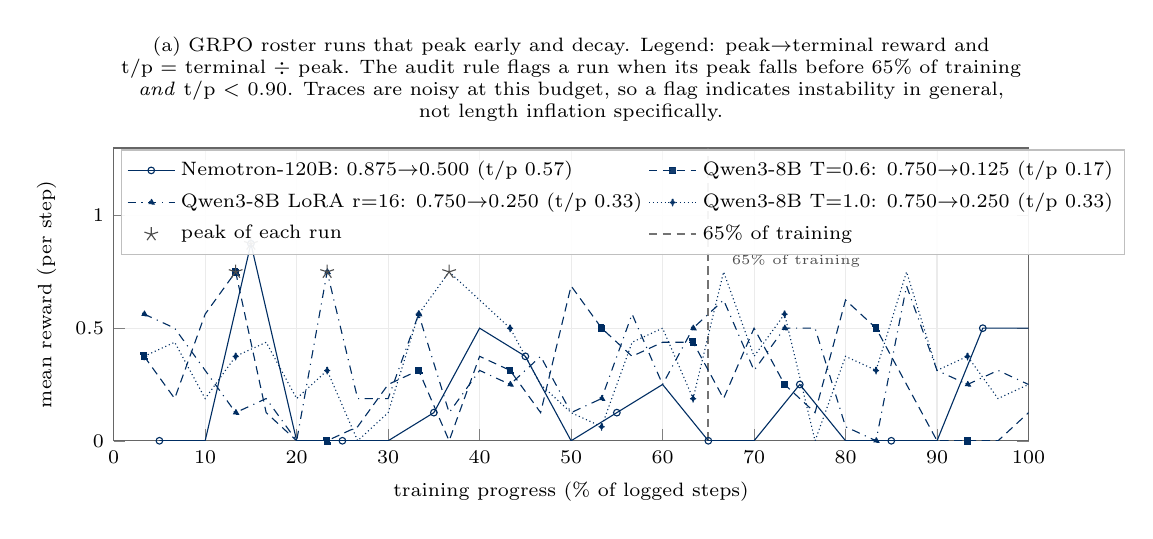
\begin{tikzpicture}
\begin{axis}[
  width=13.2cm, height=5.3cm,
  xmin=0, xmax=100, ymin=0, ymax=1.30,
  xlabel={training progress (\% of logged steps)},
  ylabel={mean reward (per step)},
  tick label style={font=\scriptsize},
  label style={font=\scriptsize},
  title style={font=\scriptsize, align=center},
  title={(a) GRPO roster runs that peak early and decay. Legend: peak$\rightarrow$terminal reward and\\ t/p $=$ terminal $\div$ peak. The audit rule flags a run when its peak falls before 65\% of training\\ \emph{and} t/p $<$ 0.90. Traces are noisy at this budget, so a flag indicates instability in general,\\ not length inflation specifically.},
  grid=major, grid style={draw=black!8},
  axis line style={black!60},
  legend style={at={(0.008,0.995)}, anchor=north west, font=\scriptsize,
                draw=black!25, fill=white, fill opacity=0.92, text opacity=1,
                inner sep=2pt, row sep=0.8pt, legend columns=2, legend cell align=left},
]

  \draw[black!55, densely dashed, thick] (axis cs:65,0) -- (axis cs:65,1.30);
  \node[anchor=west, font=\tiny, text=black!70] at (axis cs:66.5,0.80) {65\% of training};
  \addplot[solid,mark=o, pesblue, mark size=1.2pt, mark repeat=2] coordinates {(5.000,0.0000) (10.000,0.0000) (15.000,0.8750) (20.000,0.0000) (25.000,0.0000) (30.000,0.0000) (35.000,0.1250) (40.000,0.5000) (45.000,0.3750) (50.000,0.0000) (55.000,0.1250) (60.000,0.2500) (65.000,0.0000) (70.000,0.0000) (75.000,0.2500) (80.000,0.0000) (85.000,0.0000) (90.000,0.0000) (95.000,0.5000) (100.000,0.5000)};
  \addlegendentry{Nemotron-120B: 0.875$\rightarrow$0.500 (t/p 0.57)}
  \addplot[densely dashed,mark=square*, pesblue, mark size=1.2pt, mark repeat=3] coordinates {(3.333,0.3750) (6.667,0.1875) (10.000,0.5625) (13.333,0.7500) (16.667,0.1250) (20.000,0.0000) (23.333,0.0000) (26.667,0.0625) (30.000,0.2500) (33.333,0.3125) (36.667,0.0000) (40.000,0.3750) (43.333,0.3125) (46.667,0.1250) (50.000,0.6875) (53.333,0.5000) (56.667,0.3750) (60.000,0.4375) (63.333,0.4375) (66.667,0.1875) (70.000,0.5000) (73.333,0.2500) (76.667,0.1250) (80.000,0.6250) (83.333,0.5000) (86.667,0.2500) (90.000,0.0000) (93.333,0.0000) (96.667,0.0000) (100.000,0.1250)};
  \addlegendentry{Qwen3-8B T=0.6: 0.750$\rightarrow$0.125 (t/p 0.17)}
  \addplot[dash dot,mark=triangle*, pesblue, mark size=1.2pt, mark repeat=3] coordinates {(3.333,0.5625) (6.667,0.5000) (10.000,0.3125) (13.333,0.1250) (16.667,0.1875) (20.000,0.0000) (23.333,0.7500) (26.667,0.1875) (30.000,0.1875) (33.333,0.5625) (36.667,0.1250) (40.000,0.3125) (43.333,0.2500) (46.667,0.3750) (50.000,0.1250) (53.333,0.1875) (56.667,0.5625) (60.000,0.2500) (63.333,0.5000) (66.667,0.6250) (70.000,0.3125) (73.333,0.5000) (76.667,0.5000) (80.000,0.0625) (83.333,0.0000) (86.667,0.6875) (90.000,0.3125) (93.333,0.2500) (96.667,0.3125) (100.000,0.2500)};
  \addlegendentry{Qwen3-8B LoRA r=16: 0.750$\rightarrow$0.250 (t/p 0.33)}
  \addplot[densely dotted,mark=diamond*, pesblue, mark size=1.2pt, mark repeat=3] coordinates {(3.333,0.3750) (6.667,0.4375) (10.000,0.1875) (13.333,0.3750) (16.667,0.4375) (20.000,0.1875) (23.333,0.3125) (26.667,0.0000) (30.000,0.1250) (33.333,0.5625) (36.667,0.7500) (40.000,0.6250) (43.333,0.5000) (46.667,0.2500) (50.000,0.1250) (53.333,0.0625) (56.667,0.4375) (60.000,0.5000) (63.333,0.1875) (66.667,0.7500) (70.000,0.3750) (73.333,0.5625) (76.667,0.0000) (80.000,0.3750) (83.333,0.3125) (86.667,0.7500) (90.000,0.3125) (93.333,0.3750) (96.667,0.1875) (100.000,0.2500)};
  \addlegendentry{Qwen3-8B T=1.0: 0.750$\rightarrow$0.250 (t/p 0.33)}
  \addplot[only marks, mark=star, mark size=2.6pt, draw=black!70, fill=warn] coordinates {(15.000,0.8750) (13.333,0.7500) (23.333,0.7500) (36.667,0.7500)};
  \addlegendentry{peak of each run}
  \addlegendimage{black!55, densely dashed, thick}
  \addlegendentry{65\% of training}
\end{axis}
\end{tikzpicture}
\vspace{1.5ex}
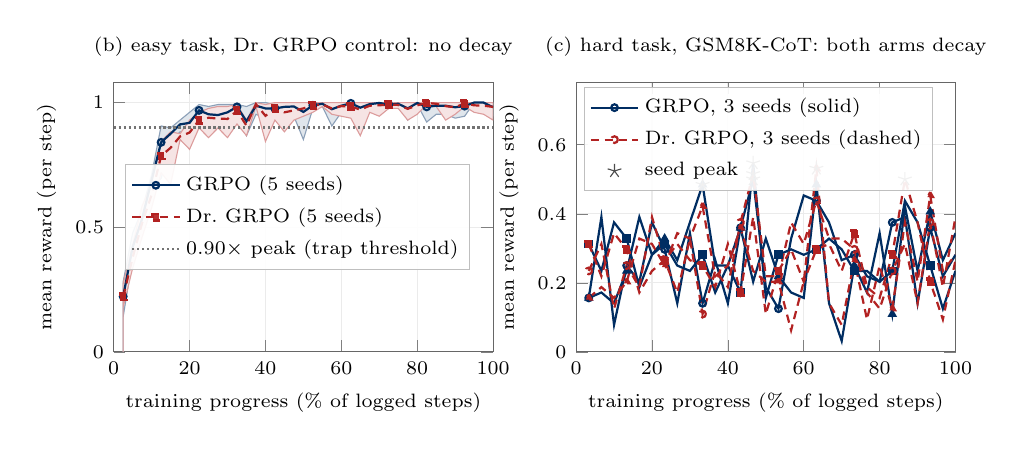
\begin{tikzpicture}
\begin{groupplot}[
  group style={group size=2 by 1, horizontal sep=30pt},
  width=6.4cm, height=5.0cm,
  xmin=0, xmax=100,
  xlabel={training progress (\% of logged steps)},
  ylabel={mean reward (per step)},
  tick label style={font=\scriptsize},
  label style={font=\scriptsize},
  title style={font=\scriptsize, align=center},
  grid=major, grid style={draw=black!8},
  axis line style={black!60},
]
\nextgroupplot[ymin=0, ymax=1.08,
  title={(b) easy task, Dr.\ GRPO control: no decay},
  legend style={at={(0.03,0.50)}, anchor=west, font=\scriptsize, draw=black!25,
                fill=white, fill opacity=0.92, text opacity=1, inner sep=2pt, row sep=0.8pt, legend cell align=left}]
  \addplot[draw=pesblue!45, fill=pesblue!12, thin, forget plot] coordinates {(2.500,0.2812) (5.000,0.4766) (7.500,0.5703) (10.000,0.7109) (12.500,0.9062) (15.000,0.8984) (17.500,0.9297) (20.000,0.9609) (22.500,0.9922) (25.000,0.9844) (27.500,0.9922) (30.000,0.9922) (32.500,0.9922) (35.000,0.9844) (37.500,1.0000) (40.000,1.0000) (42.500,0.9922) (45.000,1.0000) (47.500,1.0000) (50.000,1.0000) (52.500,1.0000) (55.000,1.0000) (57.500,1.0000) (60.000,1.0000) (62.500,1.0000) (65.000,1.0000) (67.500,1.0000) (70.000,1.0000) (72.500,1.0000) (75.000,1.0000) (77.500,1.0000) (80.000,1.0000) (82.500,1.0000) (85.000,1.0000) (87.500,1.0000) (90.000,1.0000) (92.500,1.0000) (95.000,1.0000) (97.500,1.0000) (100.000,1.0000) (100.000,0.9453) (97.500,1.0000) (95.000,1.0000) (92.500,0.9453) (90.000,0.9375) (87.500,0.9531) (85.000,0.9531) (82.500,0.9219) (80.000,0.9922) (77.500,0.9297) (75.000,0.9922) (72.500,0.9766) (70.000,0.9922) (67.500,0.9688) (65.000,0.9297) (62.500,0.9922) (60.000,0.9609) (57.500,0.9062) (55.000,0.9844) (52.500,0.9766) (50.000,0.8516) (47.500,0.9453) (45.000,0.9609) (42.500,0.9297) (40.000,0.9375) (37.500,0.9531) (35.000,0.8672) (32.500,0.9609) (30.000,0.9375) (27.500,0.9062) (25.000,0.9062) (22.500,0.9531) (20.000,0.8750) (17.500,0.8828) (15.000,0.8438) (12.500,0.6953) (10.000,0.6641) (7.500,0.5078) (5.000,0.3750) (2.500,0.1406)} \closedcycle;
  \addplot[draw=bad!45, fill=bad!12, thin, forget plot] coordinates {(2.500,0.2734) (5.000,0.4297) (7.500,0.5859) (10.000,0.6719) (12.500,0.8438) (15.000,0.8828) (17.500,0.8750) (20.000,0.9297) (22.500,0.9609) (25.000,0.9766) (27.500,0.9844) (30.000,0.9844) (32.500,0.9922) (35.000,0.9297) (37.500,1.0000) (40.000,0.9922) (42.500,1.0000) (45.000,1.0000) (47.500,1.0000) (50.000,1.0000) (52.500,1.0000) (55.000,1.0000) (57.500,1.0000) (60.000,1.0000) (62.500,1.0000) (65.000,1.0000) (67.500,1.0000) (70.000,1.0000) (72.500,1.0000) (75.000,1.0000) (77.500,1.0000) (80.000,1.0000) (82.500,1.0000) (85.000,1.0000) (87.500,1.0000) (90.000,1.0000) (92.500,1.0000) (95.000,1.0000) (97.500,1.0000) (100.000,1.0000) (100.000,0.9297) (97.500,0.9531) (95.000,0.9609) (92.500,0.9844) (90.000,0.9531) (87.500,0.9297) (85.000,0.9844) (82.500,0.9922) (80.000,0.9531) (77.500,0.9297) (75.000,0.9766) (72.500,0.9766) (70.000,0.9453) (67.500,0.9609) (65.000,0.8672) (62.500,0.9375) (60.000,0.9453) (57.500,0.9531) (55.000,0.9844) (52.500,0.9609) (50.000,0.9453) (47.500,0.9297) (45.000,0.8828) (42.500,0.9297) (40.000,0.8438) (37.500,0.9844) (35.000,0.8672) (32.500,0.9141) (30.000,0.8594) (27.500,0.8984) (25.000,0.8594) (22.500,0.8984) (20.000,0.8125) (17.500,0.8516) (15.000,0.6719) (12.500,0.7188) (10.000,0.5781) (7.500,0.4609) (5.000,0.3359) (2.500,0.1797)} \closedcycle;
  \addplot[pesblue, thick, mark=o, mark size=1.2pt, mark repeat=4] coordinates {(2.500,0.2219) (5.000,0.4203) (7.500,0.5344) (10.000,0.6891) (12.500,0.8406) (15.000,0.8750) (17.500,0.9125) (20.000,0.9187) (22.500,0.9688) (25.000,0.9531) (27.500,0.9500) (30.000,0.9609) (32.500,0.9828) (35.000,0.9250) (37.500,0.9875) (40.000,0.9766) (42.500,0.9766) (45.000,0.9828) (47.500,0.9844) (50.000,0.9625) (52.500,0.9891) (55.000,0.9953) (57.500,0.9734) (60.000,0.9875) (62.500,0.9969) (65.000,0.9797) (67.500,0.9938) (70.000,0.9984) (72.500,0.9922) (75.000,0.9953) (77.500,0.9766) (80.000,0.9984) (82.500,0.9828) (85.000,0.9875) (87.500,0.9875) (90.000,0.9812) (92.500,0.9859) (95.000,1.0000) (97.500,1.0000) (100.000,0.9812)};
  \addlegendentry{GRPO (5 seeds)}
  \addplot[bad, thick, densely dashed, mark=square*, mark size=1.2pt, mark repeat=4] coordinates {(2.500,0.2203) (5.000,0.3781) (7.500,0.5172) (10.000,0.6297) (12.500,0.7859) (15.000,0.8187) (17.500,0.8641) (20.000,0.8797) (22.500,0.9297) (25.000,0.9391) (27.500,0.9359) (30.000,0.9344) (32.500,0.9672) (35.000,0.9078) (37.500,0.9938) (40.000,0.9469) (42.500,0.9766) (45.000,0.9609) (47.500,0.9688) (50.000,0.9766) (52.500,0.9891) (55.000,0.9922) (57.500,0.9766) (60.000,0.9859) (62.500,0.9844) (65.000,0.9719) (67.500,0.9875) (70.000,0.9891) (72.500,0.9922) (75.000,0.9906) (77.500,0.9750) (80.000,0.9891) (82.500,0.9984) (85.000,0.9953) (87.500,0.9859) (90.000,0.9812) (92.500,0.9969) (95.000,0.9891) (97.500,0.9875) (100.000,0.9828)};
  \addlegendentry{Dr.\ GRPO (5 seeds)}
  \addplot[black!55, densely dotted, thick] coordinates {(0,0.90) (100,0.90)};
  \addlegendentry{$0.90\times$ peak (trap threshold)}
\nextgroupplot[ymin=0, ymax=0.78,
  title={(c) hard task, GSM8K-CoT: both arms decay},
  legend style={at={(0.02,0.985)}, anchor=north west, font=\scriptsize, draw=black!25,
                fill=white, fill opacity=0.92, text opacity=1, inner sep=2pt, row sep=0.8pt, legend cell align=left}]
  \addplot[pesblue, thick, mark=o, mark size=1.2pt, mark repeat=3] coordinates {(3.333,0.1562) (6.667,0.3906) (10.000,0.0781) (13.333,0.2500) (16.667,0.2031) (20.000,0.3750) (23.333,0.2969) (26.667,0.1406) (30.000,0.3438) (33.333,0.1406) (36.667,0.2656) (40.000,0.1406) (43.333,0.3594) (46.667,0.5000) (50.000,0.1875) (53.333,0.1250) (56.667,0.3281) (60.000,0.4531) (63.333,0.4375) (66.667,0.3750) (70.000,0.2656) (73.333,0.2812) (76.667,0.2188) (80.000,0.2031) (83.333,0.3750) (86.667,0.3906) (90.000,0.1406) (93.333,0.3594) (96.667,0.2188) (100.000,0.2812)};
  \addlegendentry{GRPO, 3 seeds (solid)}
  \addplot[pesblue, thick, mark=square*, mark size=1.2pt, mark repeat=3, forget plot] coordinates {(3.333,0.3125) (6.667,0.2344) (10.000,0.3750) (13.333,0.3281) (16.667,0.1875) (20.000,0.2812) (23.333,0.3125) (26.667,0.2500) (30.000,0.2344) (33.333,0.2812) (36.667,0.1719) (40.000,0.2500) (43.333,0.1719) (46.667,0.5469) (50.000,0.1562) (53.333,0.2812) (56.667,0.2969) (60.000,0.2812) (63.333,0.2969) (66.667,0.3281) (70.000,0.2969) (73.333,0.2344) (76.667,0.2344) (80.000,0.2031) (83.333,0.2344) (86.667,0.4375) (90.000,0.3750) (93.333,0.2500) (96.667,0.1250) (100.000,0.2344)};
  \addplot[pesblue, thick, mark=triangle*, mark size=1.2pt, mark repeat=3, forget plot] coordinates {(3.333,0.1562) (6.667,0.1719) (10.000,0.1406) (13.333,0.2344) (16.667,0.3906) (20.000,0.2812) (23.333,0.3281) (26.667,0.2656) (30.000,0.3750) (33.333,0.4844) (36.667,0.2500) (40.000,0.2500) (43.333,0.3594) (46.667,0.2031) (50.000,0.3281) (53.333,0.2188) (56.667,0.1719) (60.000,0.1562) (63.333,0.4844) (66.667,0.1406) (70.000,0.0312) (73.333,0.2500) (76.667,0.1719) (80.000,0.3438) (83.333,0.1094) (86.667,0.4219) (90.000,0.2344) (93.333,0.4062) (96.667,0.2656) (100.000,0.3438)};
  \addplot[bad, thick, densely dashed, mark=o, mark size=1.2pt, mark repeat=3] coordinates {(3.333,0.2344) (6.667,0.3125) (10.000,0.1250) (13.333,0.2500) (16.667,0.1875) (20.000,0.3906) (23.333,0.2656) (26.667,0.1719) (30.000,0.3281) (33.333,0.1094) (36.667,0.2344) (40.000,0.1875) (43.333,0.3750) (46.667,0.5156) (50.000,0.2188) (53.333,0.2188) (56.667,0.3750) (60.000,0.3125) (63.333,0.4375) (66.667,0.3281) (70.000,0.3281) (73.333,0.2969) (76.667,0.1719) (80.000,0.1250) (83.333,0.2344) (86.667,0.3125) (90.000,0.1406) (93.333,0.3750) (96.667,0.1875) (100.000,0.3906)};
  \addlegendentry{Dr.\ GRPO, 3 seeds (dashed)}
  \addplot[bad, thick, densely dashed, mark=square*, mark size=1.2pt, mark repeat=3, forget plot] coordinates {(3.333,0.3125) (6.667,0.2188) (10.000,0.3438) (13.333,0.2969) (16.667,0.1719) (20.000,0.2344) (23.333,0.2656) (26.667,0.3125) (30.000,0.2656) (33.333,0.2500) (36.667,0.1875) (40.000,0.3125) (43.333,0.1719) (46.667,0.3906) (50.000,0.1094) (53.333,0.2344) (56.667,0.2969) (60.000,0.2031) (63.333,0.2969) (66.667,0.3125) (70.000,0.2344) (73.333,0.3438) (76.667,0.1875) (80.000,0.1562) (83.333,0.2812) (86.667,0.5000) (90.000,0.3750) (93.333,0.2031) (96.667,0.0938) (100.000,0.2656)};
  \addplot[bad, thick, densely dashed, mark=triangle*, mark size=1.2pt, mark repeat=3, forget plot] coordinates {(3.333,0.1562) (6.667,0.1875) (10.000,0.1562) (13.333,0.2031) (16.667,0.3281) (20.000,0.3125) (23.333,0.2500) (26.667,0.3438) (30.000,0.3281) (33.333,0.4219) (36.667,0.2188) (40.000,0.2500) (43.333,0.3594) (46.667,0.2344) (50.000,0.2031) (53.333,0.2031) (56.667,0.0625) (60.000,0.2031) (63.333,0.5312) (66.667,0.1406) (70.000,0.0781) (73.333,0.2656) (76.667,0.0938) (80.000,0.2500) (83.333,0.1250) (86.667,0.3750) (90.000,0.2031) (93.333,0.4531) (96.667,0.2344) (100.000,0.2812)};
  \addplot[only marks, mark=star, mark size=2.6pt, draw=black!70, fill=warn] coordinates {(46.667,0.5000) (46.667,0.5469) (33.333,0.4844) (46.667,0.5156) (86.667,0.5000) (63.333,0.5312)};
  \addlegendentry{seed peak}
\end{groupplot}
\end{tikzpicture}
\vspace{1pt}
\parbox{15.2cm}{\scriptsize\raggedright
(b) easy-task control (0.5B, 40 steps, 5 seeds/arm): per-seed terminal/peak $= 0.97$--$1.00$, so the peak-then-decay rule is met by \emph{neither} arm; mean length \emph{falls} $7.6\rightarrow4.5$ (GRPO) and $7.3\rightarrow4.5$ (Dr.\ GRPO) --- no length inflation.\par
\vspace{1pt}
(c) hard task, GSM8K-CoT (1.5B, 30 steps, 3 seeds/arm): peaks at 33--47\% of training (GRPO) and 47--87\% (Dr.\ GRPO); last-10 reward $0.26$ / $0.25$, far below peak; length $196\rightarrow167$ vs $196\rightarrow181$ tokens; marker shape $=$ seed (circle 42, square 123, triangle 456).}
}
\end{document}